% *********************************************************************
% © 2010–2026 Jeremy Sylvestre
%
% Permission is granted to copy, distribute and/or modify this document
% under the terms of the GNU Free Documentation License, Version 1.3 or
% any later version published by the Free Software Foundation; with no
% Invariant Sections, no Front-Cover Texts, and no Back-Cover Texts. A
% copy of the license is included in the appendix entitled “GNU Free
% Documentation License” that appears in the output document of this
% PreTeXt source code. All trademarks™ are the registered® marks of
% their respective owners.
%
% *********************************************************************

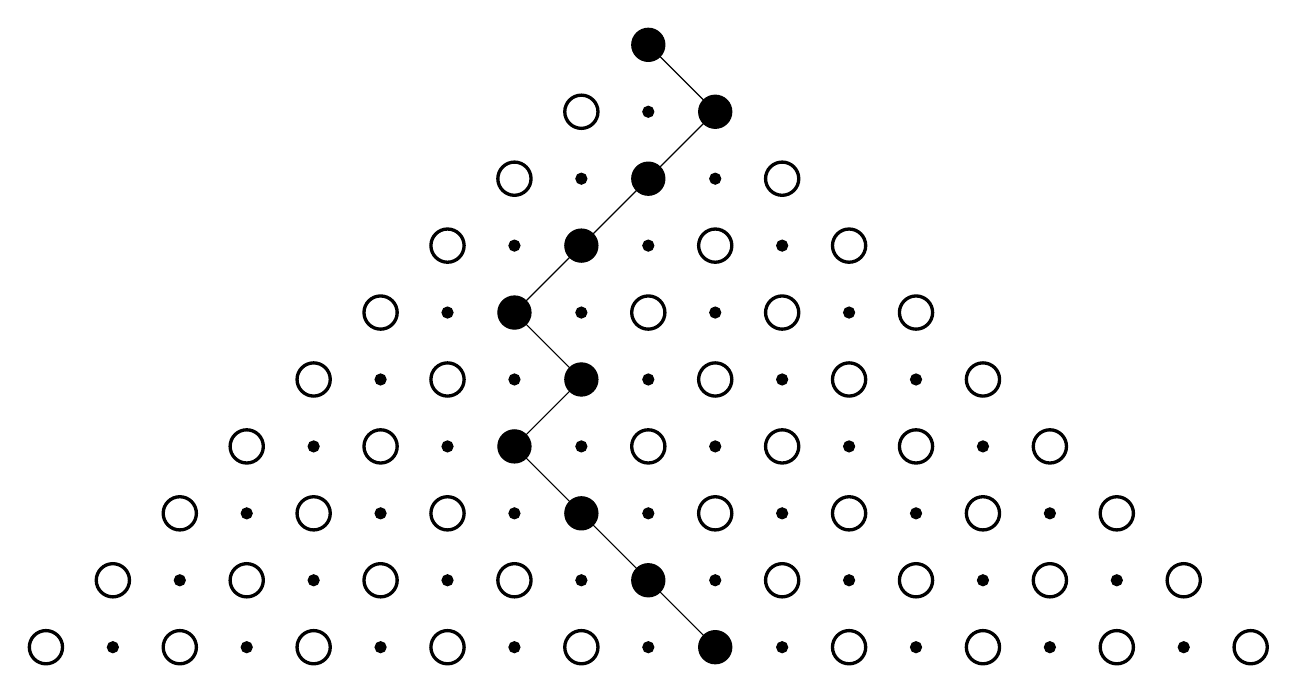
\begin{tikzpicture}[
	scale=0.85,
	pathposition/.style={ circle, draw, very thick, inner sep=0pt, minimum size=12pt },
	usedpathposition/.style={ circle, draw, fill, inner sep=0pt, minimum size=12pt },
	positiondivider/.style={ circle, draw, fill, inner sep=0pt, minimum size=4pt }
]
	\draw[thin] (0,6) to (1,5) to (-2,2) to (-1,1) to (-2,0) to (-1,-1) to (0,-2) to (1,-3);

	\node[usedpathposition] at (0,6) {};
	\node[pathposition] at (-1,5) {};
	\node[positiondivider] at (0,5) {};
	\node[usedpathposition] at (1,5) {};
	\foreach \x in {-2,2} { \node[pathposition] at (\x,4) {}; }
	\foreach \x in {-1,1} { \node[positiondivider] at (\x,4) {}; }
	\node[usedpathposition] at (0,4) {};
	\foreach \x in {-3,1,3} { \node[pathposition] at (\x,3) {}; }
	\foreach \x in {-2,0,2} { \node[positiondivider] at (\x,3) {}; }
	\node[usedpathposition] at (-1,3) {};
	\foreach \x in {-4,0,2,4} { \node[pathposition] at (\x,2) {}; }
	\foreach \x in {-3,-1,1,3} { \node[positiondivider] at (\x,2) {}; }
	\node[usedpathposition] at (-2,2) {};
	\foreach \x in {-5,-3,1,3,5} { \node[pathposition] at (\x,1) {}; }
	\foreach \x in {-4,-2,0,2,4} { \node[positiondivider] at (\x,1) {}; }
	\node[usedpathposition] at (-1,1) {};
	\foreach \x in {-6,-4,0,2,4,6} { \node[pathposition] at (\x,0) {}; }
	\foreach \x in {-5,-3,-1,1,3,5} { \node[positiondivider] at (\x,0) {}; }
	\node[usedpathposition] at (-2,0) {};
	\foreach \x in {-7,-5,-3,1,3,5,7} { \node[pathposition] at (\x,-1) {}; }
	\foreach \x in {-6,-4,-2,0,2,4,6} { \node[positiondivider] at (\x,-1) {}; }
	\node[usedpathposition] at (-1,-1) {};
	\foreach \x in {-8,-6,-4,-2,2,4,6,8} { \node[pathposition] at (\x,-2) {}; }
	\foreach \x in {-7,-5,-3,-1,1,3,5,7} { \node[positiondivider] at (\x,-2) {}; }
	\node[usedpathposition] at (0,-2) {};
	\foreach \x in {-9,-7,-5,-3,-1,3,5,7,9} { \node[pathposition] at (\x,-3) {}; }
	\foreach \x in {-8,-6,-4,-2,0,2,4,6,8} { \node[positiondivider] at (\x,-3) {}; }
	\node[usedpathposition] at (1,-3) {};

\end{tikzpicture}
